
\documentclass[12pt]{amsart}
\usepackage{amsmath}
\usepackage{amssymb}
\usepackage{./.sty/titlesec}
\usepackage{graphicx}
\usepackage{subcaption}
\usepackage{listings}
\usepackage{csvsimple}
\usepackage{./.sty/appendix}


\graphicspath{ {../analysis/plots} }


\titlelabel{\thetitle.\quad}


\title{
  {Time Series Analysis of Twitter Data}\\
}


\author{
  Matthew Tiger \\
}


\begin{document}


\maketitle
\newpage


\begin{section}{Introduction}
  The authors were tasked by the client with finding the solution to the following
family of differential equations
\[
  \begin{cases}
    -u''(x) + c u(x) = f(x) \\
    0 \leq x \leq 1 \\
    u(0) = \epsilon \\
    u(1) = \delta.
  \end{cases}
\]
Additionally, the client has also requested to be provided with a means of
plotting the solution once obtained.

Throughout this report, the above family of differential equations together with
the interval of definition and initial conditions will be represented by
$Lu = f$ where $L$ can be thought of as the differential operator for the above family.

Assumptions were placed on this family so that $c \in \mathbb{R}$ with $c > 0$
and $f \in C^k([0,1])$ for sufficiently large $k$ so that $f$ is relatively
well-behaved on the defined interval.

In this report we will detail the analytical solution to this family of
differential equations showing that the above problem is well-posed and
explain why this solution is not amenable to practical use. We therefore
provide a numerical scheme to approximate the solution to the family of
differential equations and examine the convergence, consistency and stability
of the numerical scheme. Using the solution provided by the numerical scheme,
we then explore the method for plotting the solution.

\end{section}


\begin{section}{Data}\label{data}
  In an effort to help researchers glean insight from tweets, Twitter offers
a streaming API that streams all tweets that contain a certain string.
We leverage this service to gather data surrounding the popular television
show \textit{The Walking Dead} and then measure the number of tweets that occur each
hour over a time span.

Using the programming language Python and the library \texttt{tweepy}, a popular
wrapper for the Twitter streaming API, we collected all tweets containing the
hashtag ``\#thewalkingdead'' for three weeks from 2015-11-07 21:00 EST to
2015-11-23 21:00 EST. As this television show airs Sundays at 21:00 EST,
of particular importance is the tweets occurring around this time.
We therefore restrict our measurements to 24 hours prior to and 24 hours after
the television show's airing for the above three week time frame.

These measurements give rise to the time series presented in Figure \ref{tweets_plot}.
From this plot it is clear that, due to the weekly episodic nature of the television
show, there is a seasonal component to this time series. It also appears that
there is a trend component. Thus, in order to fit a stationary time series
to the underlying data, we will need to first apply transformations to the data.

\begin{figure}[!t]
  \centerline{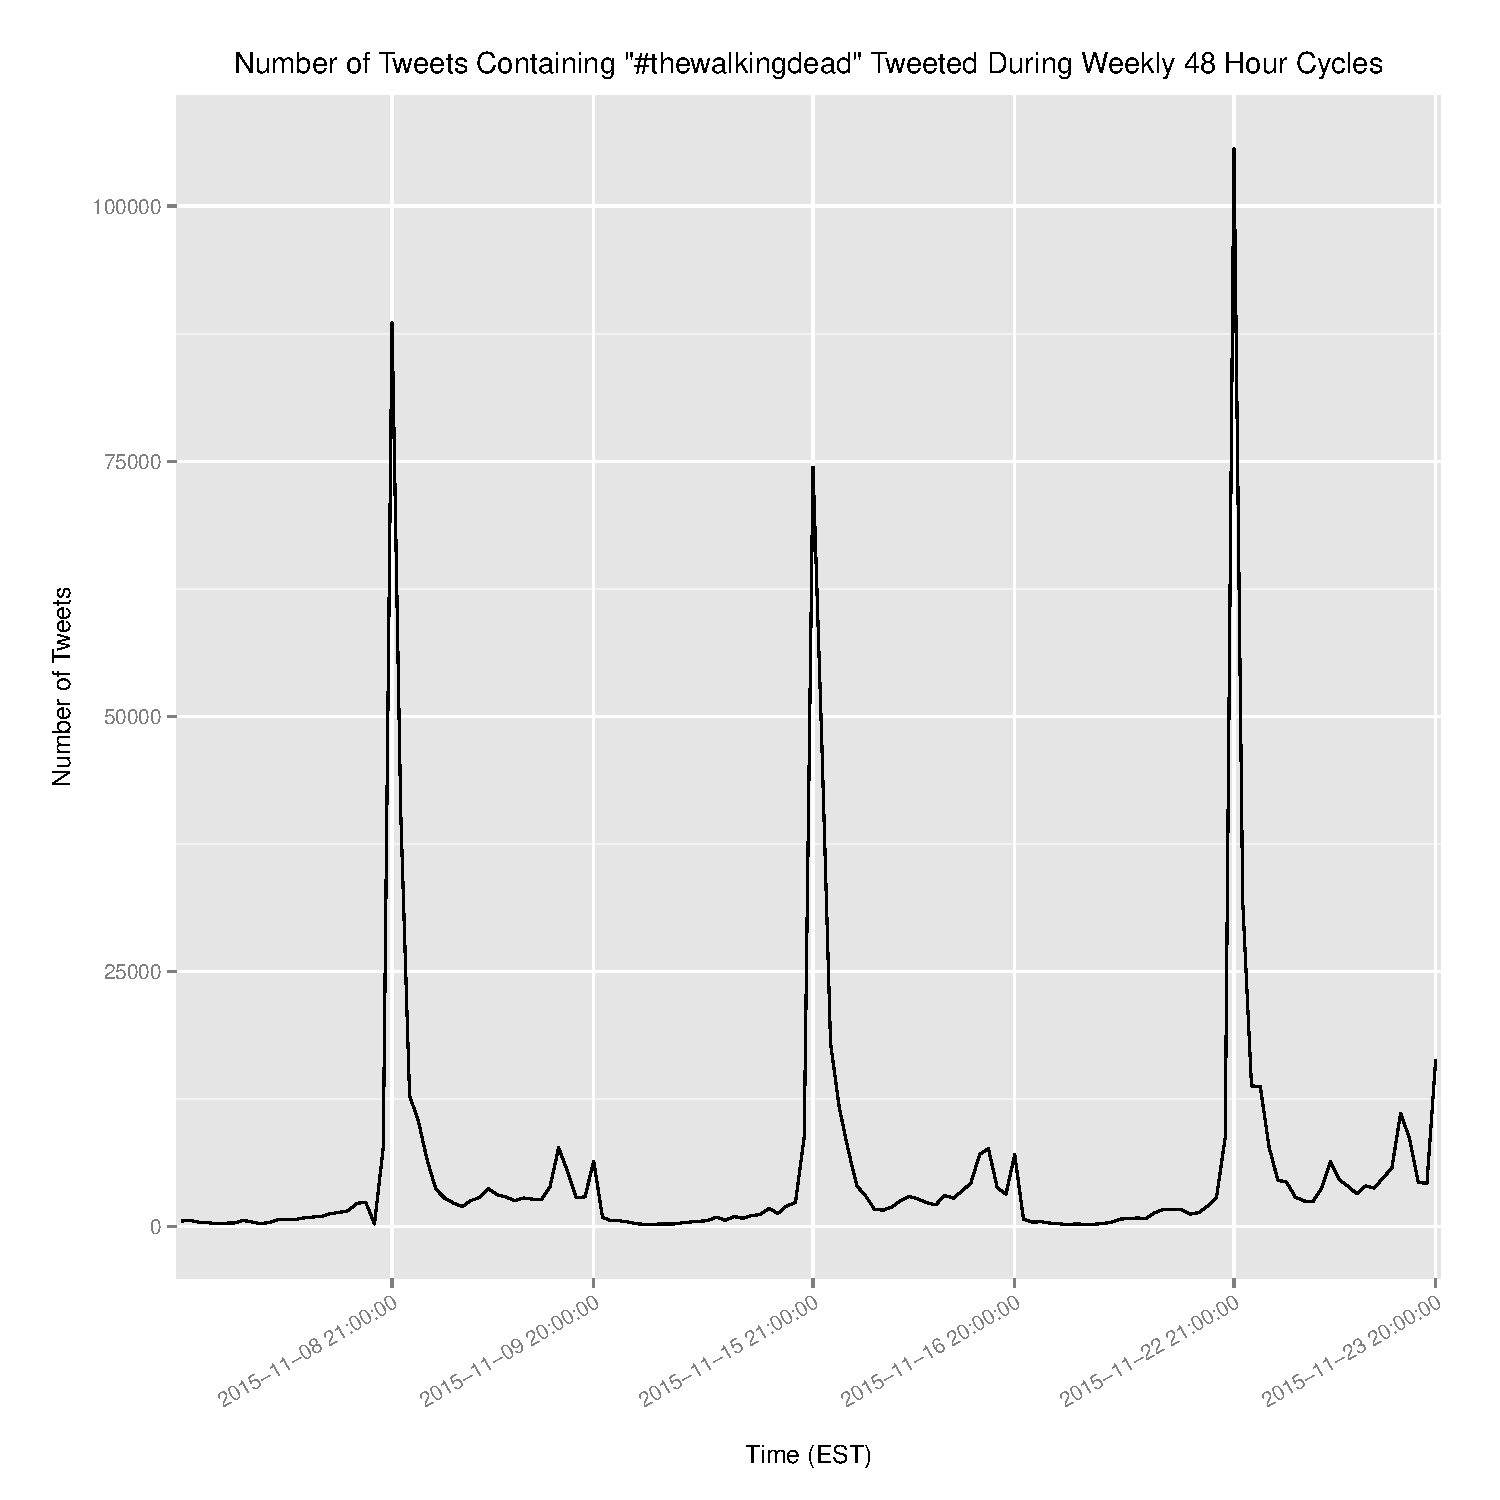
\includegraphics[scale=0.75]{../analysis/plots/tweets_plot}}
  \caption{Time series plot of number of tweets containing the hashtag
  \#thewalkingdead over three 48 hour cycles.}\label{tweets_plot}
\end{figure}

The details behind the process of fitting a stationary time series model to this data is handled in
Section \ref{model}.
\end{section}


\begin{section}{Model Fitting}\label{model}
  We now wish to fit a time series model to the data described in Section \ref{data}.
As can be seen from Figure \ref{tweets_plot}, there are seasonal and trend components
present in the underlying data set and what also appears to be non-constant variance.

Thus, we will need to apply transformations to the time series in order to determine
the underlying time series model.

\begin{subsection}{Transformations}\label{transformations}
  Let $\{X_t\}$ for $t=1,2,\dots, 144$ denote the observations
  of the time series described in Section \ref{data}. To remove the non-constant variance
  we apply the Box-Cox transformation $\log$ to the observations $\{X_t\}$ to arrive
  at the mean-corrected data $Y_t = \log(X_t) - E(\log(X_t))$ for $t=1,2,\dots, 144$.
  As can be seen from Figure \ref{log_plot}, this transformation has made the variance
  of the data constant.

  \begin{figure}[!h]
    \centerline{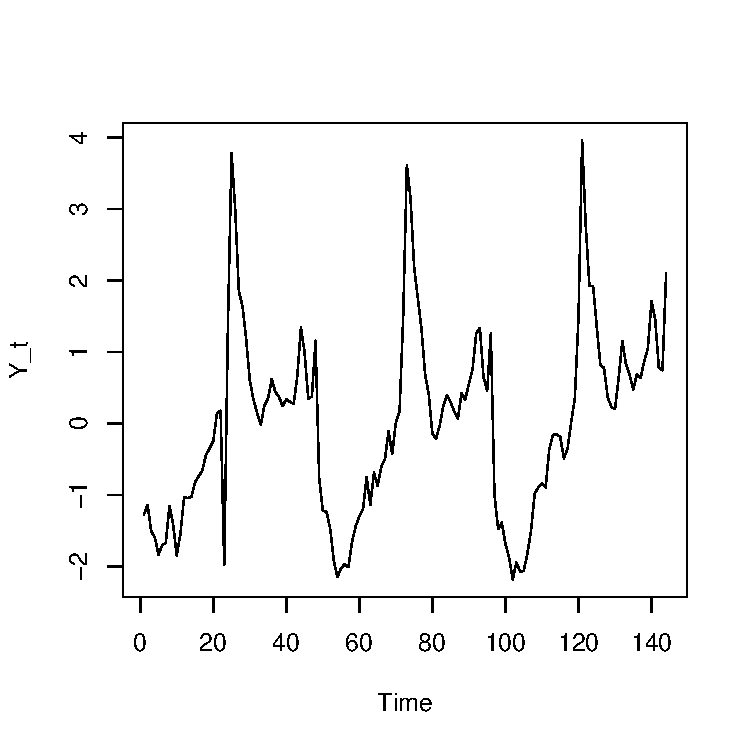
\includegraphics[scale=0.75]{../analysis/plots/log_plot}}
    \caption{Plot of Box-Cox transformed data $Y_t = \log(X_t) - E(\log(X_t))$.}\label{log_plot}
  \end{figure}

  The seasonality and trend noticed with the untransformed data is still present in
  the transformed data. Through differencing, we hope to characterize the underlying
  seasonality and trend of the data.

  Knowing that the observations come from data with a period of 48 hours, it makes sense
  to remove the seasonality by applying the differencing operator $\left(1 - B^{48}\right)$ to $Y_t$.
  Applying this transformation results in Figure \ref{seasonal_plot}.

  \begin{figure}[!h]
    \centerline{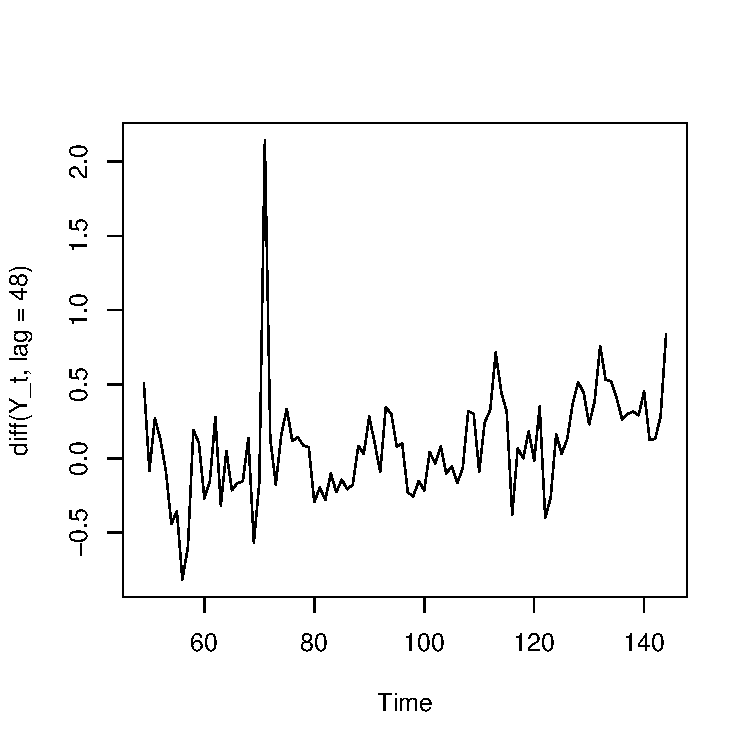
\includegraphics[scale=0.75]{../analysis/plots/seasonal_plot}}
    \caption{Plot of data $\left(1 - B^{48}\right)Y_t$.}\label{seasonal_plot}
  \end{figure}

  As can be seen from the figure, the seasonality has been removed. The plots
  of the ACF and the PACF of $\left(1 - B^{48}\right)Y_t$ are found in Figure \ref{cf_seasonal}.

  \begin{figure}[!h]
    \begin{subfigure}[b]{.48\textwidth}
      \centering
      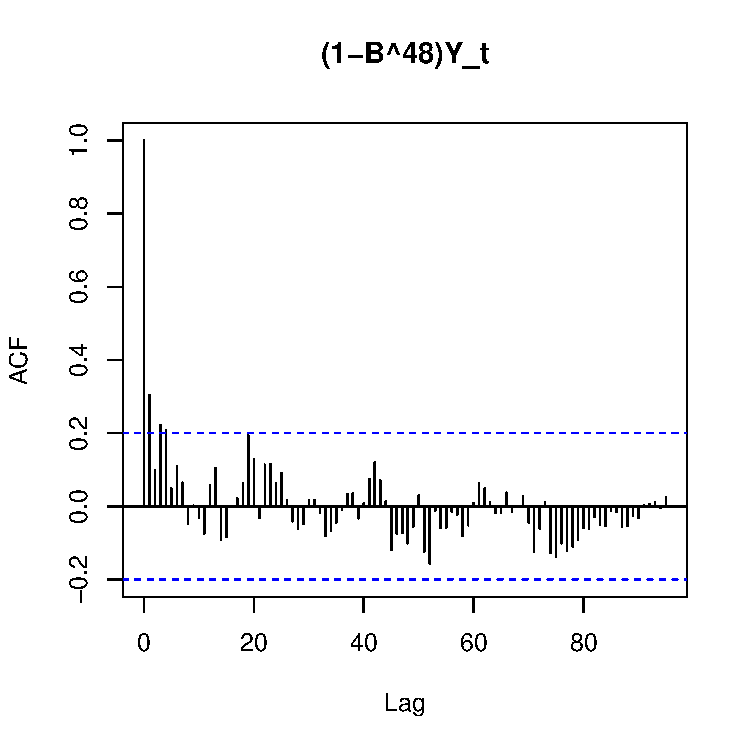
\includegraphics[scale=0.5]{../analysis/plots/seasonal_acf}
    \end{subfigure}
    \begin{subfigure}[b]{.48\textwidth}
      \centering
      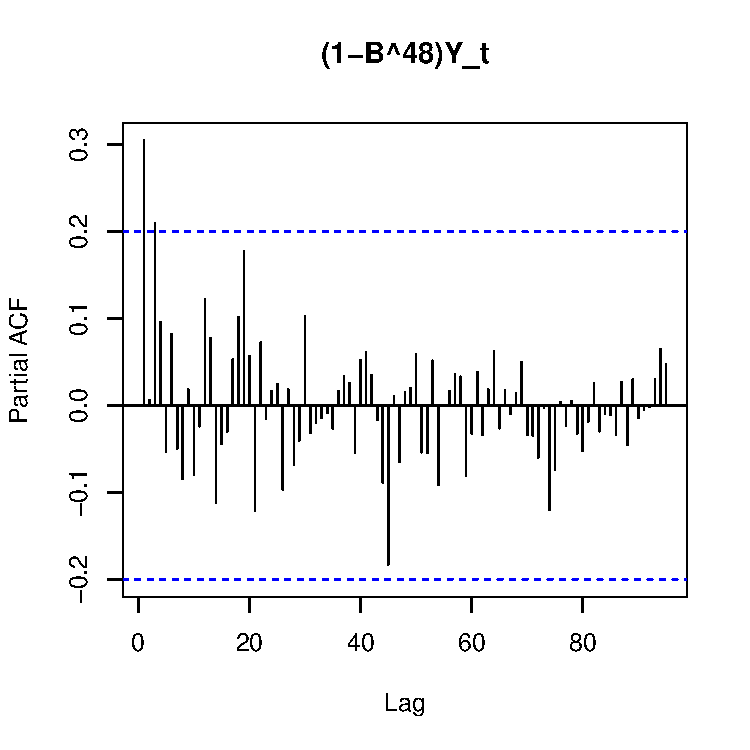
\includegraphics[scale=0.5]{../analysis/plots/seasonal_pacf}
    \end{subfigure}
    \caption{ACF and PACF of $\left(1 - B^{48}\right)Y_t$.}\label{cf_seasonal}
  \end{figure}

  These plots suggest that a seasonal AR model of order 1 or 3 may be
  appropriate as the ACF slowly decreases to 0 while the PACF stops abruptly
  after lag 3.

  However, as can also be seen in Figure \ref{seasonal_plot}, there is still a
  trend component present. This trend appears linear suggesting that applying
  the difference operator $(1 - B)$ to $\left(1 - B^{48}\right)Y_t$ will remove
  this trend. The results of applying the operator are found in Figure \ref{trend_plot}.

  \begin{figure}[!h]
    \centerline{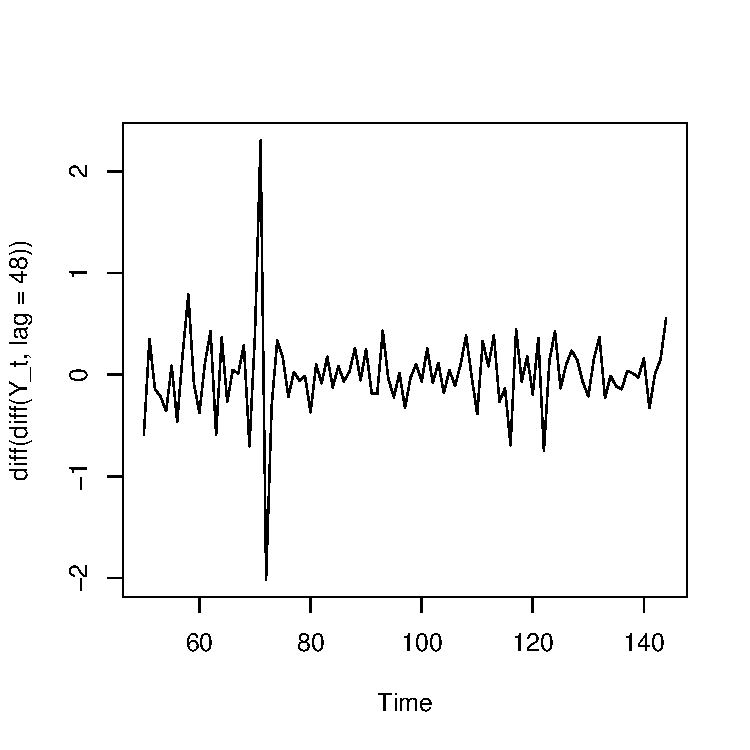
\includegraphics[scale=0.75]{../analysis/plots/trend_plot}}
    \caption{Plot of data $(1-B)\left(1 - B^{48}\right)Y_t$.}\label{trend_plot}
  \end{figure}

  The plot in Figure \ref{trend_plot} shows that the trend component.
  The plots of the ACF and the PACF of
  $(1-B)\left(1 - B^{48}\right)Y_t$ are found in Figure \ref{cf_trend}.

  \begin{figure}[!h]
    \begin{subfigure}[b]{.48\textwidth}
      \centering
      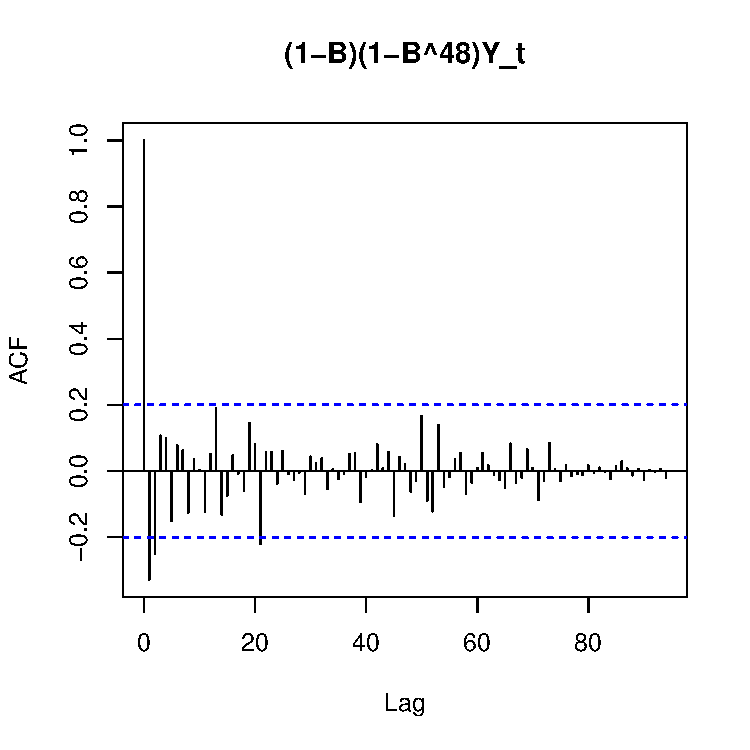
\includegraphics[scale=0.5]{../analysis/plots/trend_acf}
    \end{subfigure}
    \begin{subfigure}[b]{.48\textwidth}
      \centering
      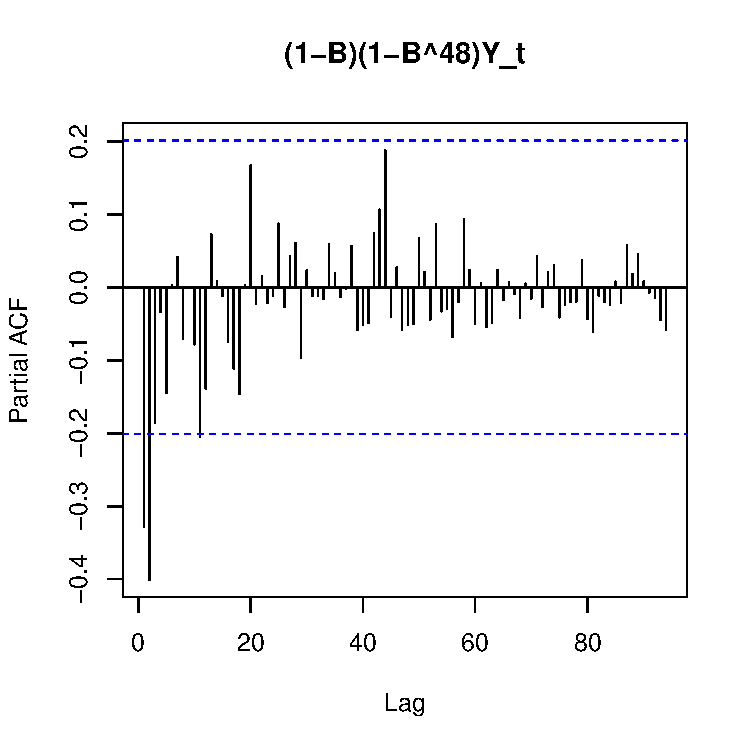
\includegraphics[scale=0.5]{../analysis/plots/trend_pacf}
    \end{subfigure}
    \caption{ACF and PACF of $(1-B)\left(1 - B^{48}\right)Y_t$.}\label{cf_trend}
  \end{figure}

  These plots suggest a possible AR model of order 2 for the trend component as the ACF
  slowly decreases to
  0 while the PACF stops abruptly after lag 2. It is also possible for an MA component
  to be present so we will investigate models of the form ARMA($p$, $q$) for $p,q=1,2$
  for the trend component.
\end{subsection}

\begin{subsection}{Model Selection}
  The findings from Section \ref{transformations} suggest fitting the data $\{Y_t\}$
  to a seasonal ARIMA model. Specifically, a model of the form
  \[
    \text{SARIMA}(p, 1, q)\times (P, 1, 0)_{48}
  \]
  where $p, q \in \{0, 1, 2\}$ and $P \in \{1, 3\}$.

  Using the programming language R, we examine the AIC statistic associated to
  each of the different possible models suggested and choose the model that
  minimizes this statistic. Due to the limitations of the available hardware,
  we were unable to fit SARIMA models to the data in which $P=3$ for such a large period.
  Thus, we present the results of testing for $P=1$ alone.

  \begin{table}[h!]
    \centering
    \def\arraystretch{1.25}
    \begin{tabular}{| p{1.5cm} | p{1.5cm} | p{2cm} |}
      \hline
      $p$ & $q$ & AIC \\
      \hline
      0 & 1 & 77.00203 \\
      0 & 2 & 75.06627 \\
      1 & 0 & 99.46614 \\
      1 & 1 & \texttt{NaN} \\
      1 & 2 & 78.04194 \\
      2 & 0 & 85.23537 \\
      2 & 1 & 77.33328 \\
      2 & 2 & 78.92953 \\
      \hline
    \end{tabular}
    \vspace{3mm}
    \caption{AIC values for different possible SARIMA$(p,1,q)\times(1,1,0)_{48}$
      models fitted to the data $Y_t = \log(X_t) - E(\log(X_t))$.}\label{aic_table}
  \end{table}

  Note that hardware limitations also prevented us from fitting a model of the
  form $\text{SARIMA}(1,1,1)\times(1,1,0)_{48}$
  to the data so that has been omitted from consideration as well. Table \ref{aic_table} suggests
  that, if we are to select a model based on minimizing the AIC statistic,
  we should choose to fit the data to a SARIMA$(0,1,2)\times(1,1,0)_{48}$ model.

  Doing so produces the following output in R:
  \begin{lstlisting}[language=R]
Coefficients:
          ma1      ma2     sar1
      -0.6768  -0.2257  -0.1586
s.e.   0.1097   0.1100   0.1441

sigma^2 estimated as 0.1152:  log likelihood = -33.53,  aic = 75.07
  \end{lstlisting}
  The above gives the associated p-values for the coefficients of the model:
  \begin{lstlisting}[language=R]
      ma1          ma2         sar1
6.878613e-10 4.021464e-02 2.709825e-01
  \end{lstlisting}

  Using a significance level of $\alpha=0.05$ suggests that the SAR(1) coefficient
  is not significant. However, removing the seasonal component and fitting the model
  to an MA(2) model results in a worse fit. Thus, we elect to keep the seasonal
  component in the model.

  Thus, we fit our data $Y_t = \log(X_t) - E(\log(X_t))$ to the model
  \begin{align}\label{sarima_model}
    Y_t = \Phi_1Y_{t-48} + Z_t + \theta_1Z_{t-1} + \theta_2Z_{t-2} \quad Z_t \sim \text{WN}(0, \sigma^2) \notag\\
    \Phi_1 = -0.1586, \quad \theta_1 = -0.6768, \quad \theta_2 = -0.2257, \quad \sigma^2 = 0.1152.
  \end{align}
  We verify that these residuals are indeed
  a white noise process by examining the plot of their ACF in Figure \ref{res_acf}.

  \begin{figure}[!h]
    \centerline{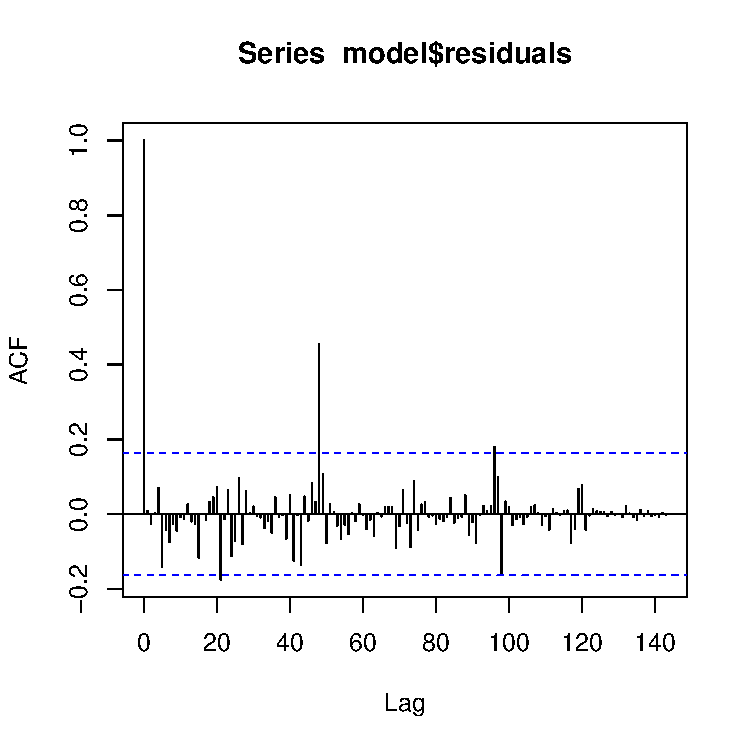
\includegraphics[scale=0.75]{../analysis/plots/res_acf}}
    \caption{Plot of ACF of $Z_t$ in \eqref{sarima_model}.}\label{res_acf}
  \end{figure}

  As almost all of the values fall within the 0-bound, we conclude that this
  process is most likely a white noise process.

\end{subsection}
\end{section}


\begin{section}{Forecasting}
  Now that we have fitted our data $\{Y_t\}$ to a suitable model, the next
reasonable step is to use the model to provide a forecast of the next 48 hour cycle
,i.e. for the time period of 2015-11-28 21:00 EST - 2015-11-30 21:00 EST.

The programming language R provides many tools to forecast data. One such tool
is the \texttt{forecast} package, which we employ. Using the model provided by
\eqref{sarima_model}, we provide the model in an acceptable form to the
function \texttt{predict} as well as the desired number of lags, e.g. 48,
and arrive at the forecasted values. As the model is for the transformed data
$Y_t = \log(X_t) - E(\log(X_t))$, we must apply the inverse transformation to the
forecasted values. Doing so gives us the table of values found in Appendix
\ref{forecast_table} along with 90\% confidence intervals. A plot of these
forecasts combined with the original data can be found in Figure \ref{forecast_plot}.

\begin{figure}[!h]
  \centerline{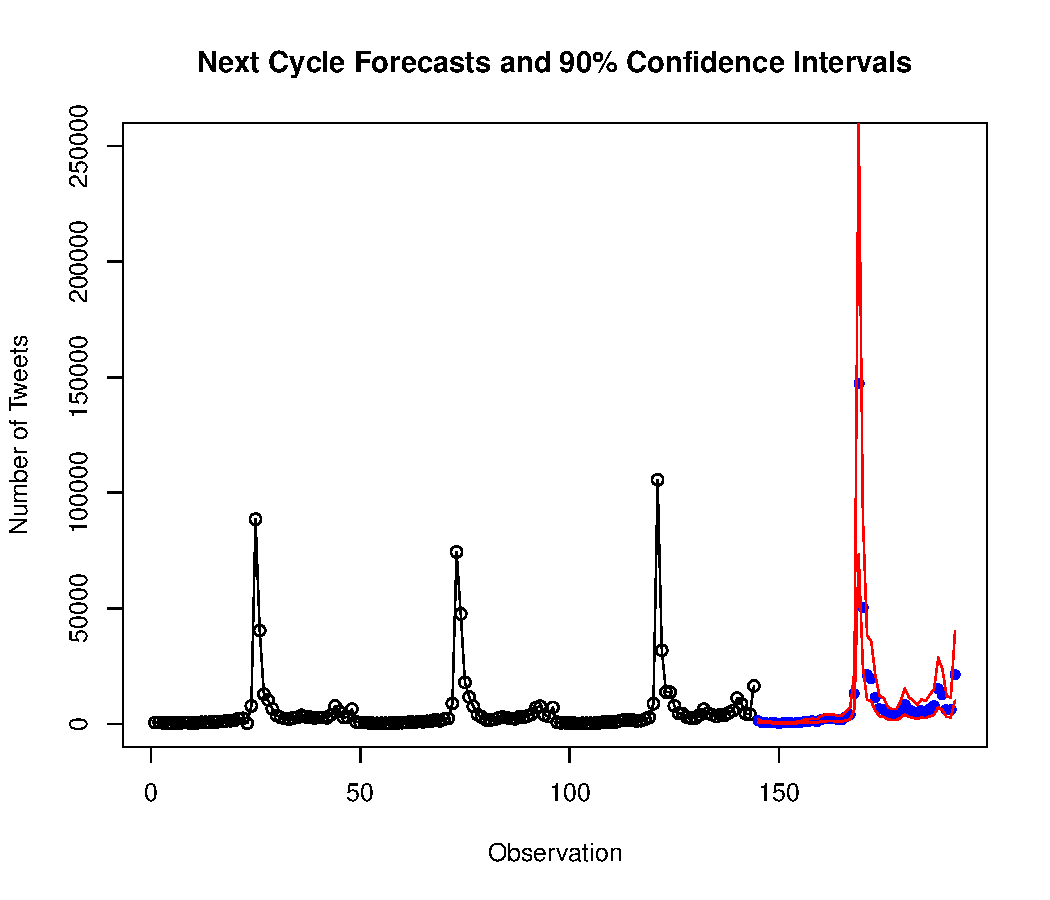
\includegraphics[scale=0.75]{../analysis/plots/forecast}}
  \caption{Plot of forecasted data for the next 48 cycle for data $X_t$.}\label{forecast_plot}
\end{figure}

The shape of the forecast seems to follow the same shape as the previous cycles
suggesting that the forecasts seem plausible. Also note the sensitivity of
the forecast at the time of interest, i.e. at 2015-11-29 21:00 EST.
\end{section}


\begin{section}{Conclusion}
  \begin{chapter}{Conclusion}

\end{chapter}
\end{section}


\newpage
\begin{appendices}
\section{Future Forecasts of Twitter Data}\label{forecast_table}
The first 24 hours of the forecasted 48 hour cycle.\\\\
\csvautotabular{../analysis/data/forecast_1.csv}
\newpage
The latter 24 hours of the forecasted 48 hour cycle.\\\\
\csvautotabular{../analysis/data/forecast_2.csv}
\end{appendices}


\end{document}
